\chapter{Motoren mit Arduino steuern}\label{ch:chapter_02}

Motoren benötigen deutlich mehr Strom, als ein Arduino-Pin sicher liefern kann. Servomotoren und Gleichstrommotoren werden deshalb über eine geeignete externe Spannungsversorgung betrieben. Deren Masse muss mit \texttt{GND} des Arduino verbunden werden, damit das Steuersignal ein gemeinsames Bezugspotential besitzt.

\begin{myattention}
Schliessen Sie einen Motor nie direkt an einen Arduino-Pin an. Prüfen Sie vor dem Einschalten die zulässige Betriebsspannung und die Stromaufnahme. Halten Sie den Roboter bei ersten Tests so fest, dass sich die Räder frei drehen können.
\end{myattention}

\section{Servomotoren}
Ein Servomotor besteht aus einem Elektromotor, einem Getriebe, einem Positionssensor und einer Regelelektronik. Anders als ein gewöhnlicher Gleichstrommotor dreht sich ein Positionsservo nicht kontinuierlich, sondern fährt einen vorgegebenen Winkel an. Viele kleine Servomotoren besitzen einen Bewegungsbereich von ungefähr \qty{0}{\degree} bis \qty{180}{\degree}.

Ein Servomotor besitzt drei Anschlüsse: Versorgungsspannung (\texttt{VCC}, meist rot), Masse (\texttt{GND}, meist braun oder schwarz) und Steuersignal (meist orange oder gelb).

\begin{figure}[ht]
	\centering
	\begin{minipage}[c]{.38\textwidth}
		\centering
		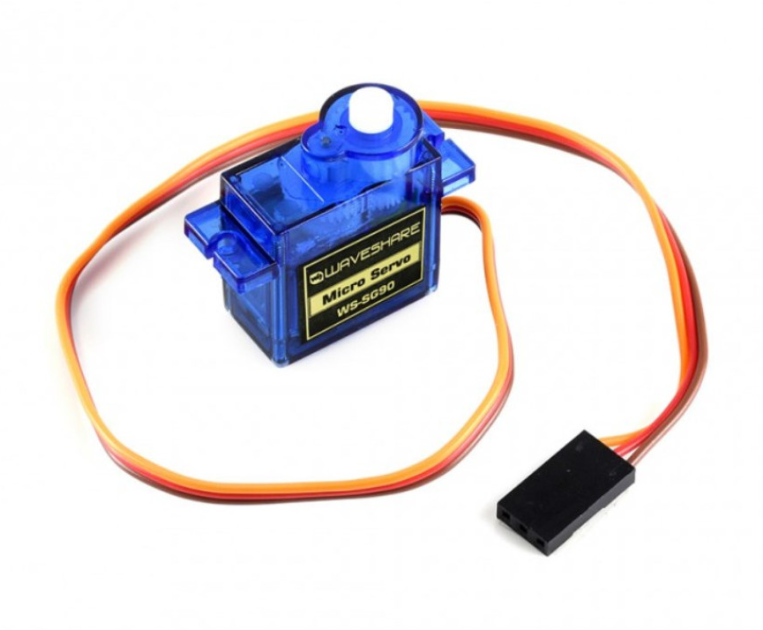
\includegraphics[width=.82\linewidth]{FF/Robotik/Skript/Abbildungen/tower_pro_micro_servo.png}
	\end{minipage}\hfill
	\begin{minipage}[c]{.57\textwidth}
		\centering
		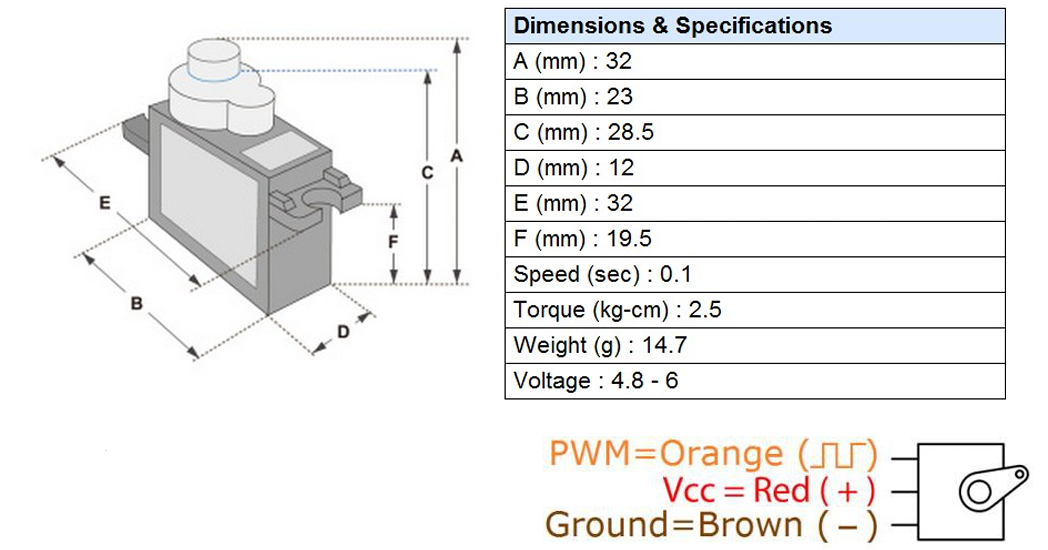
\includegraphics[width=\linewidth]{FF/Robotik/Skript/Abbildungen/sg90_servomotor_daten.png}
	\end{minipage}
	\caption{Micro-Servomotor und beispielhafte Kenndaten eines SG90-Servos.}
	\label{fig:servo-connections}
\end{figure}

Zur Ansteuerung wird die Bibliothek \texttt{Servo.h} verwendet. Sie kann bei Bedarf über die Bibliotheksverwaltung der Arduino IDE installiert werden. \Cref{fig:servo-external-supply} zeigt den Servo an einer externen Spannungsversorgung. Das Steuersignal ist mit Pin~\texttt{9} verbunden; Arduino und Batterie besitzen eine gemeinsame Masse.

\begin{figure}[ht]
	\centering
	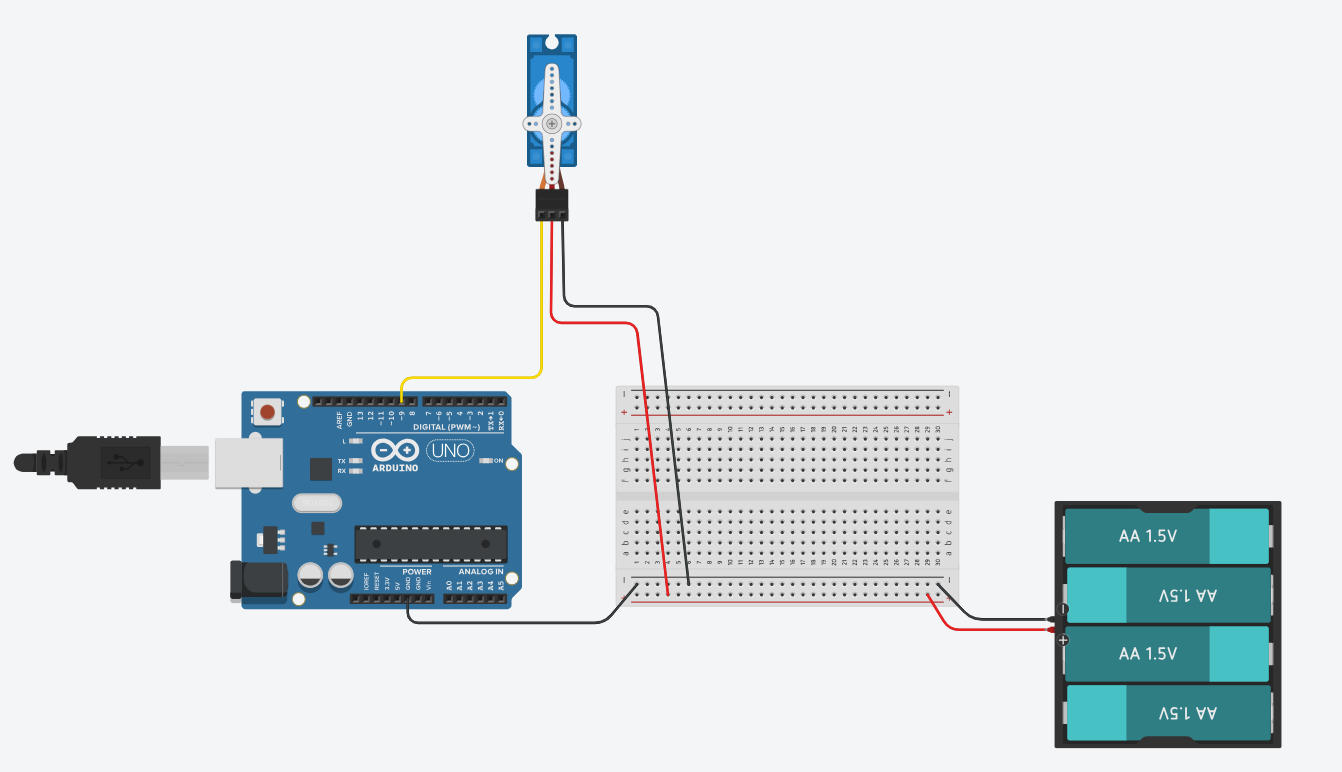
\includegraphics[width=.72\textwidth]{FF/Robotik/Skript/Abbildungen/servomotor_batterie.png}
	\caption{Servomotor mit externer Spannungsversorgung und gemeinsamer Masse.}
	\label{fig:servo-external-supply}
\end{figure}

\lstinputlisting[
	language=C++, morekeywords={setup,loop,Servo,attach,write,delay},
	columns=fullflexible, keepspaces=true, breaklines=false,
	showspaces=false, showstringspaces=false, showtabs=false, tabsize=2,
	numbers=none, basicstyle=\ttfamily\footnotesize,
	caption={Servomotor zwischen \qty{0}{\degree} und \qty{180}{\degree} schwenken},
	label={lst:servo-sweep}
]{FF/Robotik/Skript/Code/Servo_Sweep/Servo_Sweep.ino}

\begin{myexercise}
Bauen Sie die Schaltung aus \cref{fig:servo-external-supply} auf und untersuchen Sie \cref{lst:servo-sweep}.
\begin{aenum}
	\item Erklären Sie, wie das Servo-Objekt \cppinline{myServo} mit Pin~\texttt{9} verknüpft wird.
	\item Bestimmen Sie, welche Winkelwerte die beiden \cppinline{for}-Schleifen erzeugen.
	\item Übertragen Sie den Sketch und beobachten Sie die Bewegung.
	\item Verändern Sie \cppinline{delay()} in beiden Schleifen und erklären Sie die Auswirkung.
\end{aenum}
\begin{myanswer}keine Musterlösung\end{myanswer}
\end{myexercise}

\subsection{Servomotor mit einem Potentiometer steuern}
Ein Potentiometer kann als Sollwertgeber dienen. Der Messwert von $0$ bis $1023$ wird mit \cppinline{map()} auf einen Winkel von \qty{0}{\degree} bis \qty{180}{\degree} abgebildet und mit \cppinline{write()} an den Servo übergeben.

\begin{figure}[ht]
	\centering
	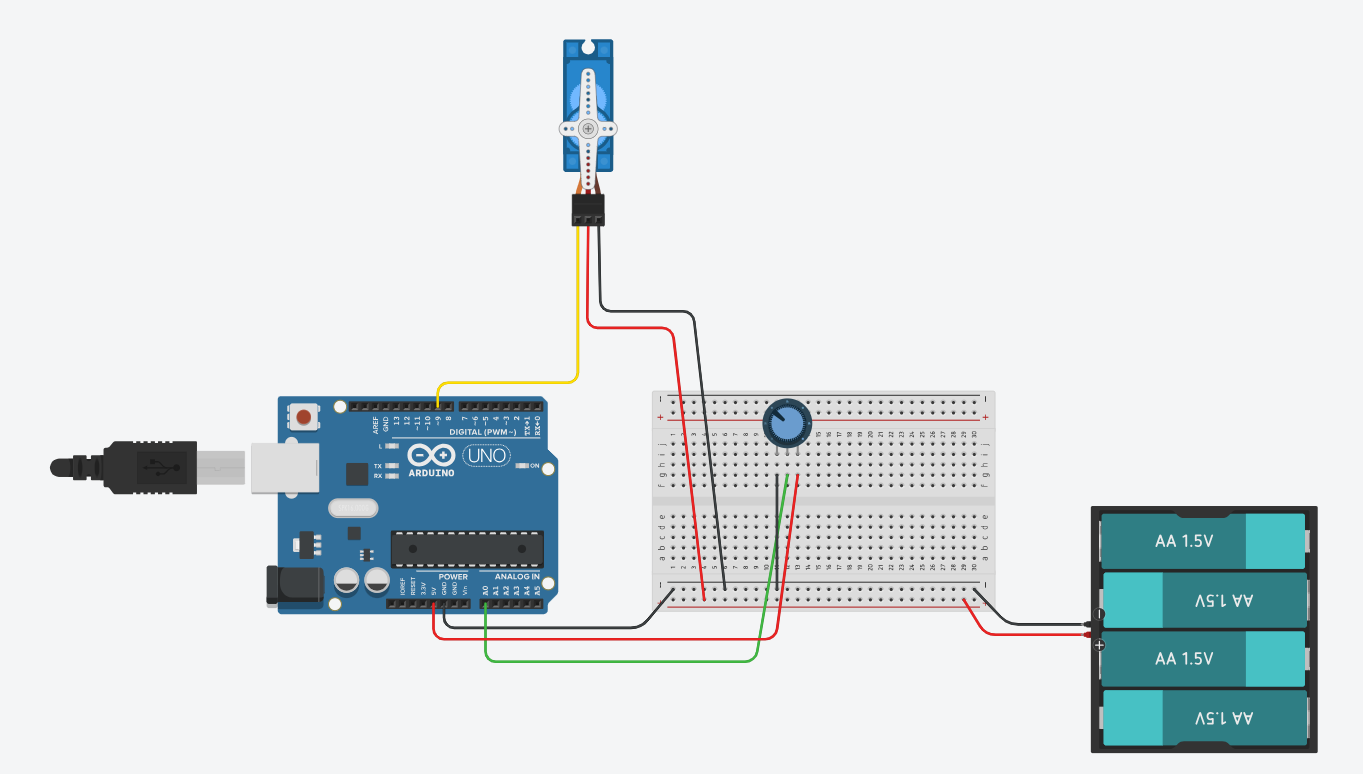
\includegraphics[width=.74\textwidth]{FF/Robotik/Skript/Abbildungen/servomotor_potentiometer_batterie.png}
	\caption{Servomotor mit externer Spannungsversorgung und Potentiometer an \texttt{A0}.}
	\label{fig:servo-potentiometer-circuit}
\end{figure}

\begin{myexercise}
Erweitern Sie den Sketch aus \cref{lst:servo-sweep}.
\begin{aenum}
	\item Bauen Sie \cref{fig:servo-potentiometer-circuit} auf und lesen Sie das Potentiometer an \texttt{A0} aus.
	\item Bilden Sie den Messwert mit \cppinline{map()} auf \qty{0}{\degree} bis \qty{180}{\degree} ab und übergeben Sie ihn mit \cppinline{write()}.
	\item Vergleichen Sie Ihre Lösung mit \emph{Datei $\rightarrow$ Beispiele $\rightarrow$ Servo $\rightarrow$ Knob}.
\end{aenum}
\begin{myanswer}keine Musterlösung\end{myanswer}
\end{myexercise}

\subsection{Steuersignal eines Servomotors}
Bei einer typischen Wiederholfrequenz von \qty{50}{\hertz} beträgt die Periodendauer \qty{20}{\milli\second}. Die Impulsbreite bestimmt die Sollposition. Je nach Modell umfasst der nutzbare Bereich beispielsweise \qtyrange{1}{2}{\milli\second} oder \qtyrange{0.5}{2.5}{\milli\second}. Anders als bei der PWM aus \cref{ch:chapter_01} ist hier die absolute Impulsdauer entscheidend.

\begin{figure}[ht]
	\centering
	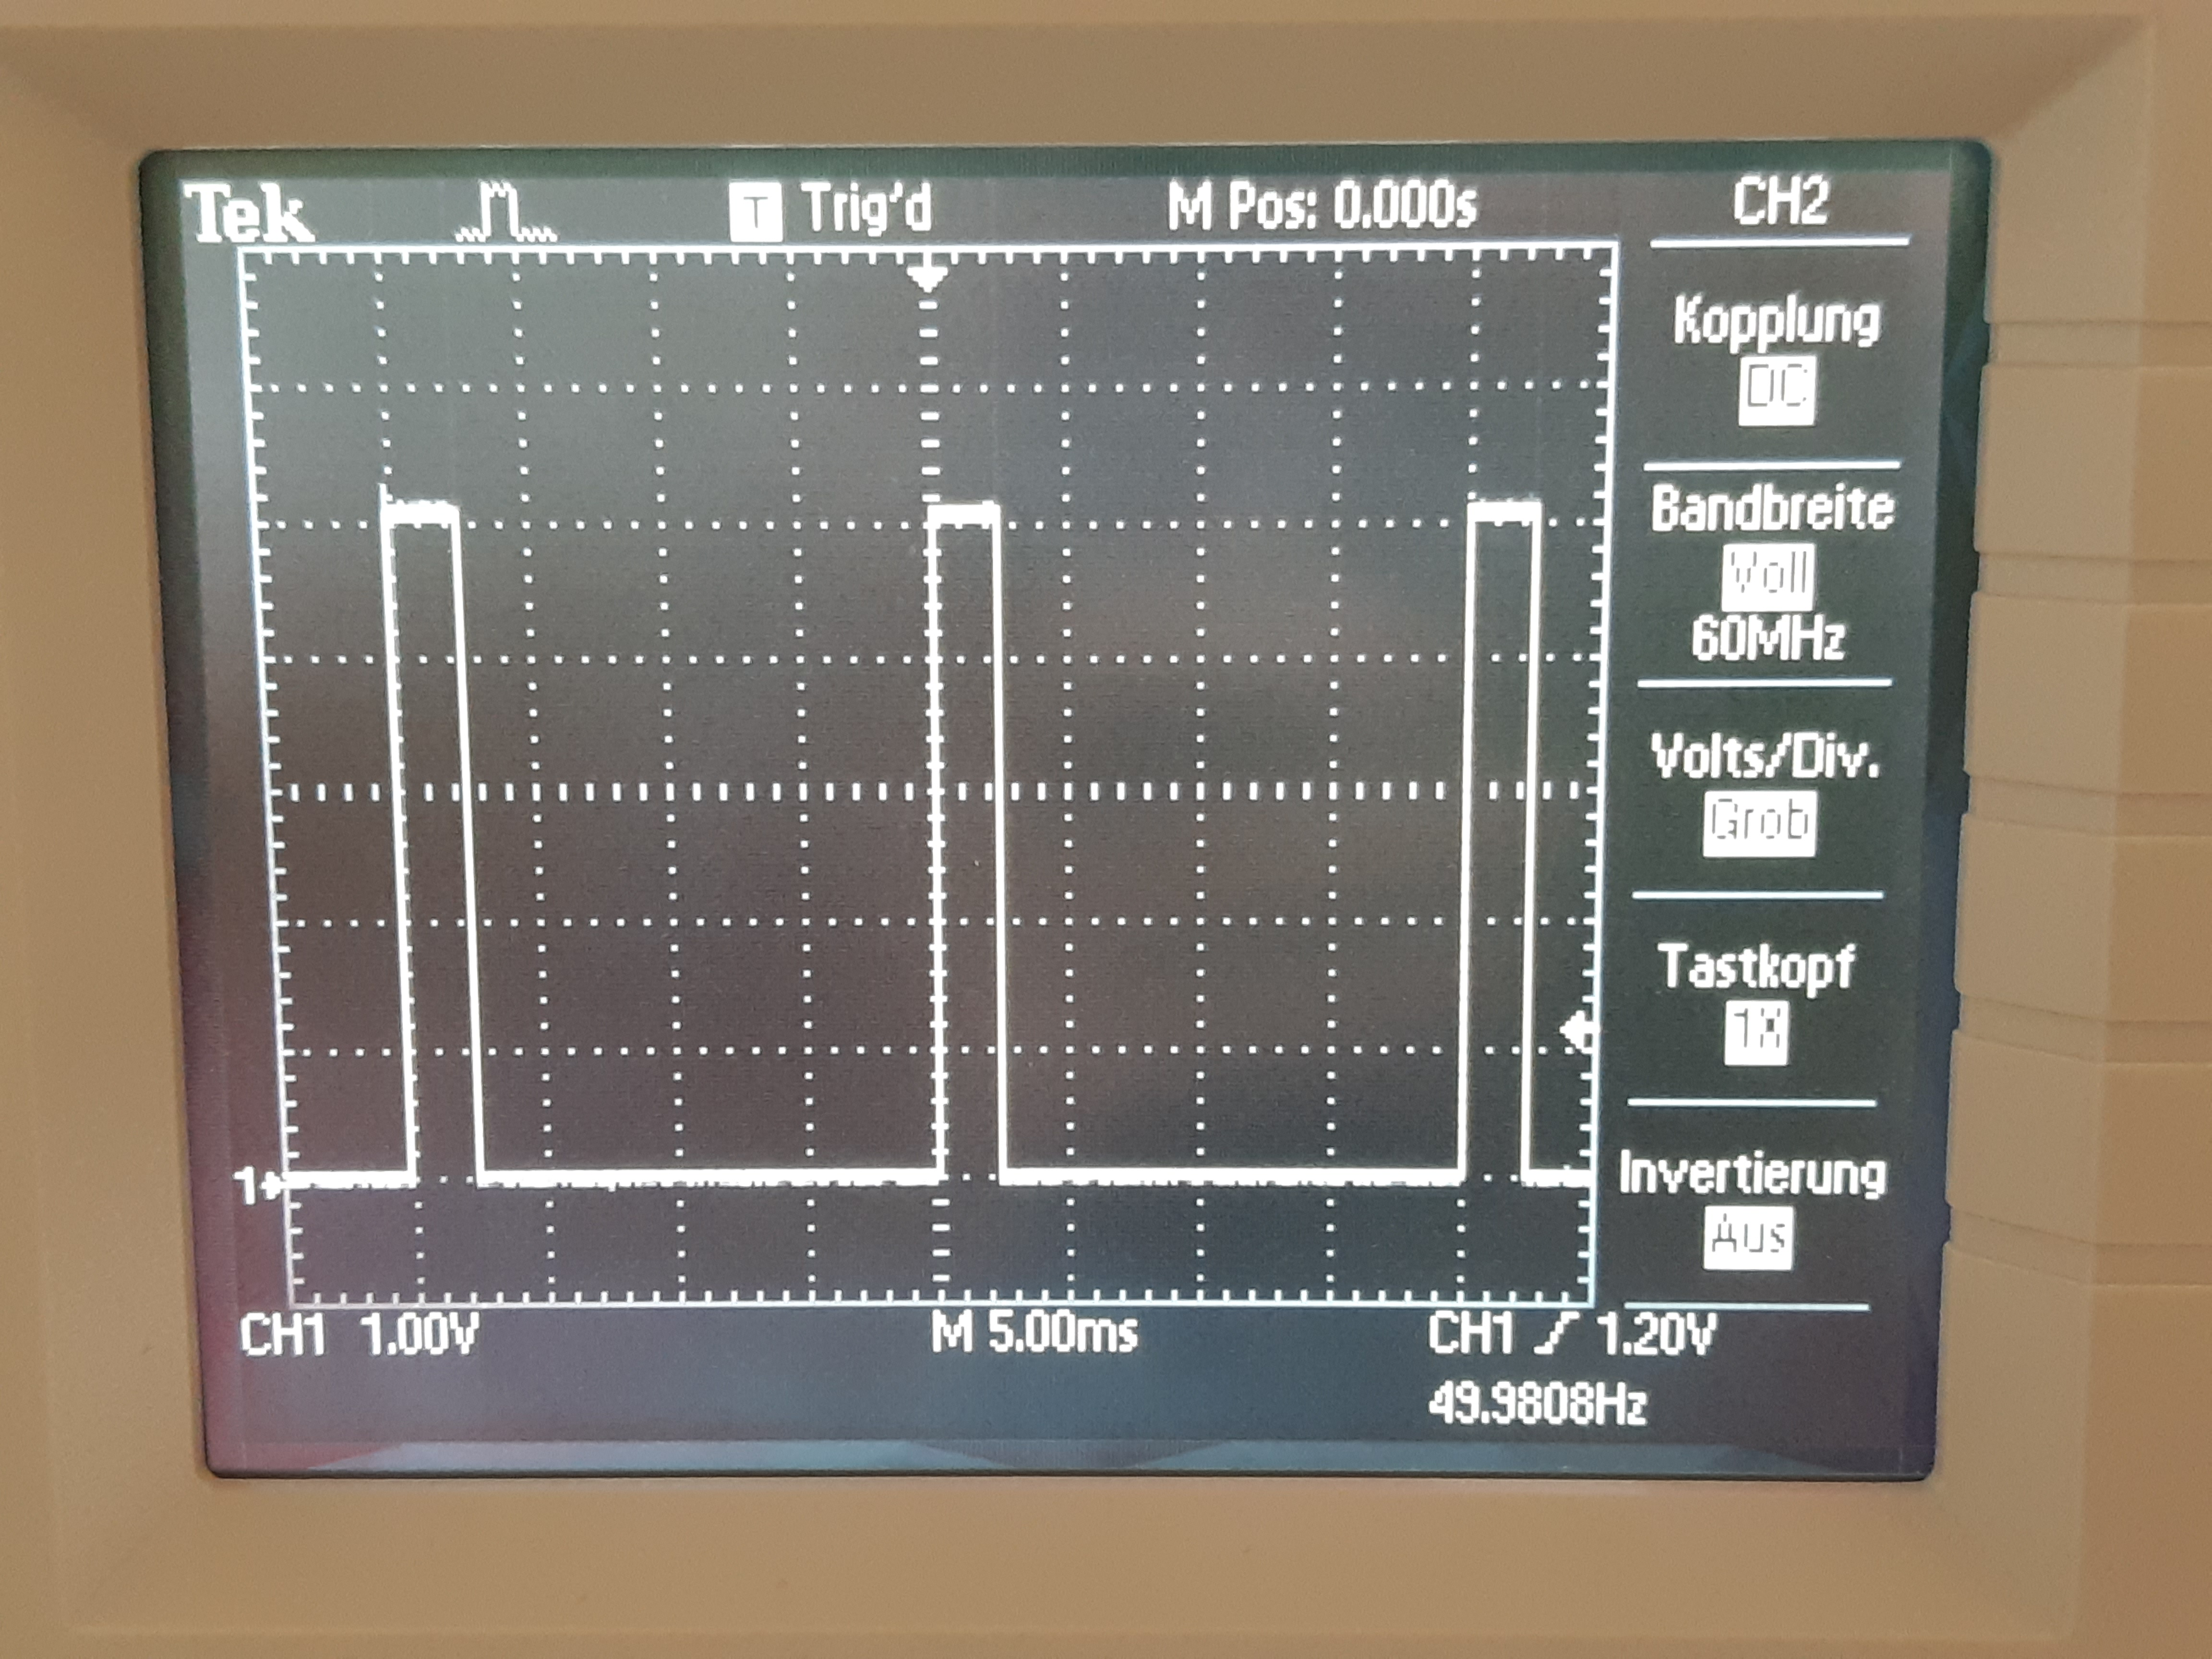
\includegraphics[width=.58\textwidth]{FF/Robotik/Skript/Abbildungen/servo_pwm_maximalwinkel.jpg}
	\caption{Mit dem Oszilloskop gemessenes Steuersignal eines Servomotors.}
	\label{fig:servo-oscilloscope-signal}
\end{figure}

\begin{myexercise}
Messen Sie bei beiden Endstellungen Periodendauer und Impulsbreite. Bestimmen Sie die Wiederholfrequenz und die Impulsbreiten für ungefähr \qty{0}{\degree} und \qty{180}{\degree}.
\begin{myanswer}keine Musterlösung\end{myanswer}
\end{myexercise}

Mit \cppinline{myServo.attach(9, minPulse, maxPulse)} lassen sich die Impulsbreiten der Endpositionen in Mikrosekunden anpassen. Verändern Sie diese nur in kleinen Schritten von \qtyrange{10}{20}{\micro\second} und nie über einen mechanischen Anschlag hinaus.

\section{Gleichstrommotoren}
Gleichstrommotoren eignen sich als Rad- oder Propellerantrieb. Da ein Arduino die Motorströme nicht direkt liefern kann, übernimmt beim Roboter ein Adafruit Motor Shield die Ansteuerung. Für \cref{lst:dc-motor-test} werden die Bibliotheken \texttt{Adafruit Motor Shield V2 Library} und \texttt{Adafruit PWM Servo Driver Library} benötigt.

\lstinputlisting[
	language=C++, morekeywords={setup,loop,begin,getMotor,run,setSpeed,Adafruit_MotorShield,Adafruit_DCMotor,FORWARD,RELEASE},
	columns=fullflexible, keepspaces=true, breaklines=true,
	showspaces=false, showstringspaces=false, showtabs=false, tabsize=2,
	numbers=none, basicstyle=\ttfamily\footnotesize,
	caption={Zwei Gleichstrommotoren mit dem Adafruit Motor Shield ansteuern},
	label={lst:dc-motor-test}
]{FF/Robotik/Skript/Code/DC_Motor_Test/DC_Motor_Test.ino}

\begin{myattention}
Verwenden Sie für \cppinline{setSpeed()} in diesem Aufbau höchstens den Wert $100$.
\end{myattention}

\begin{myexercise}
Beschreiben Sie vor dem Übertragen die erwartete Bewegung. Testen Sie den Sketch mit frei drehenden Rädern, vergleichen Sie das Ergebnis mit Ihrer Vorhersage und ändern Sie ihn so, dass die Bewegungsfolge wiederholt wird.
\begin{myanswer}keine Musterlösung\end{myanswer}
\end{myexercise}

\begin{figure}[ht]
	\centering
	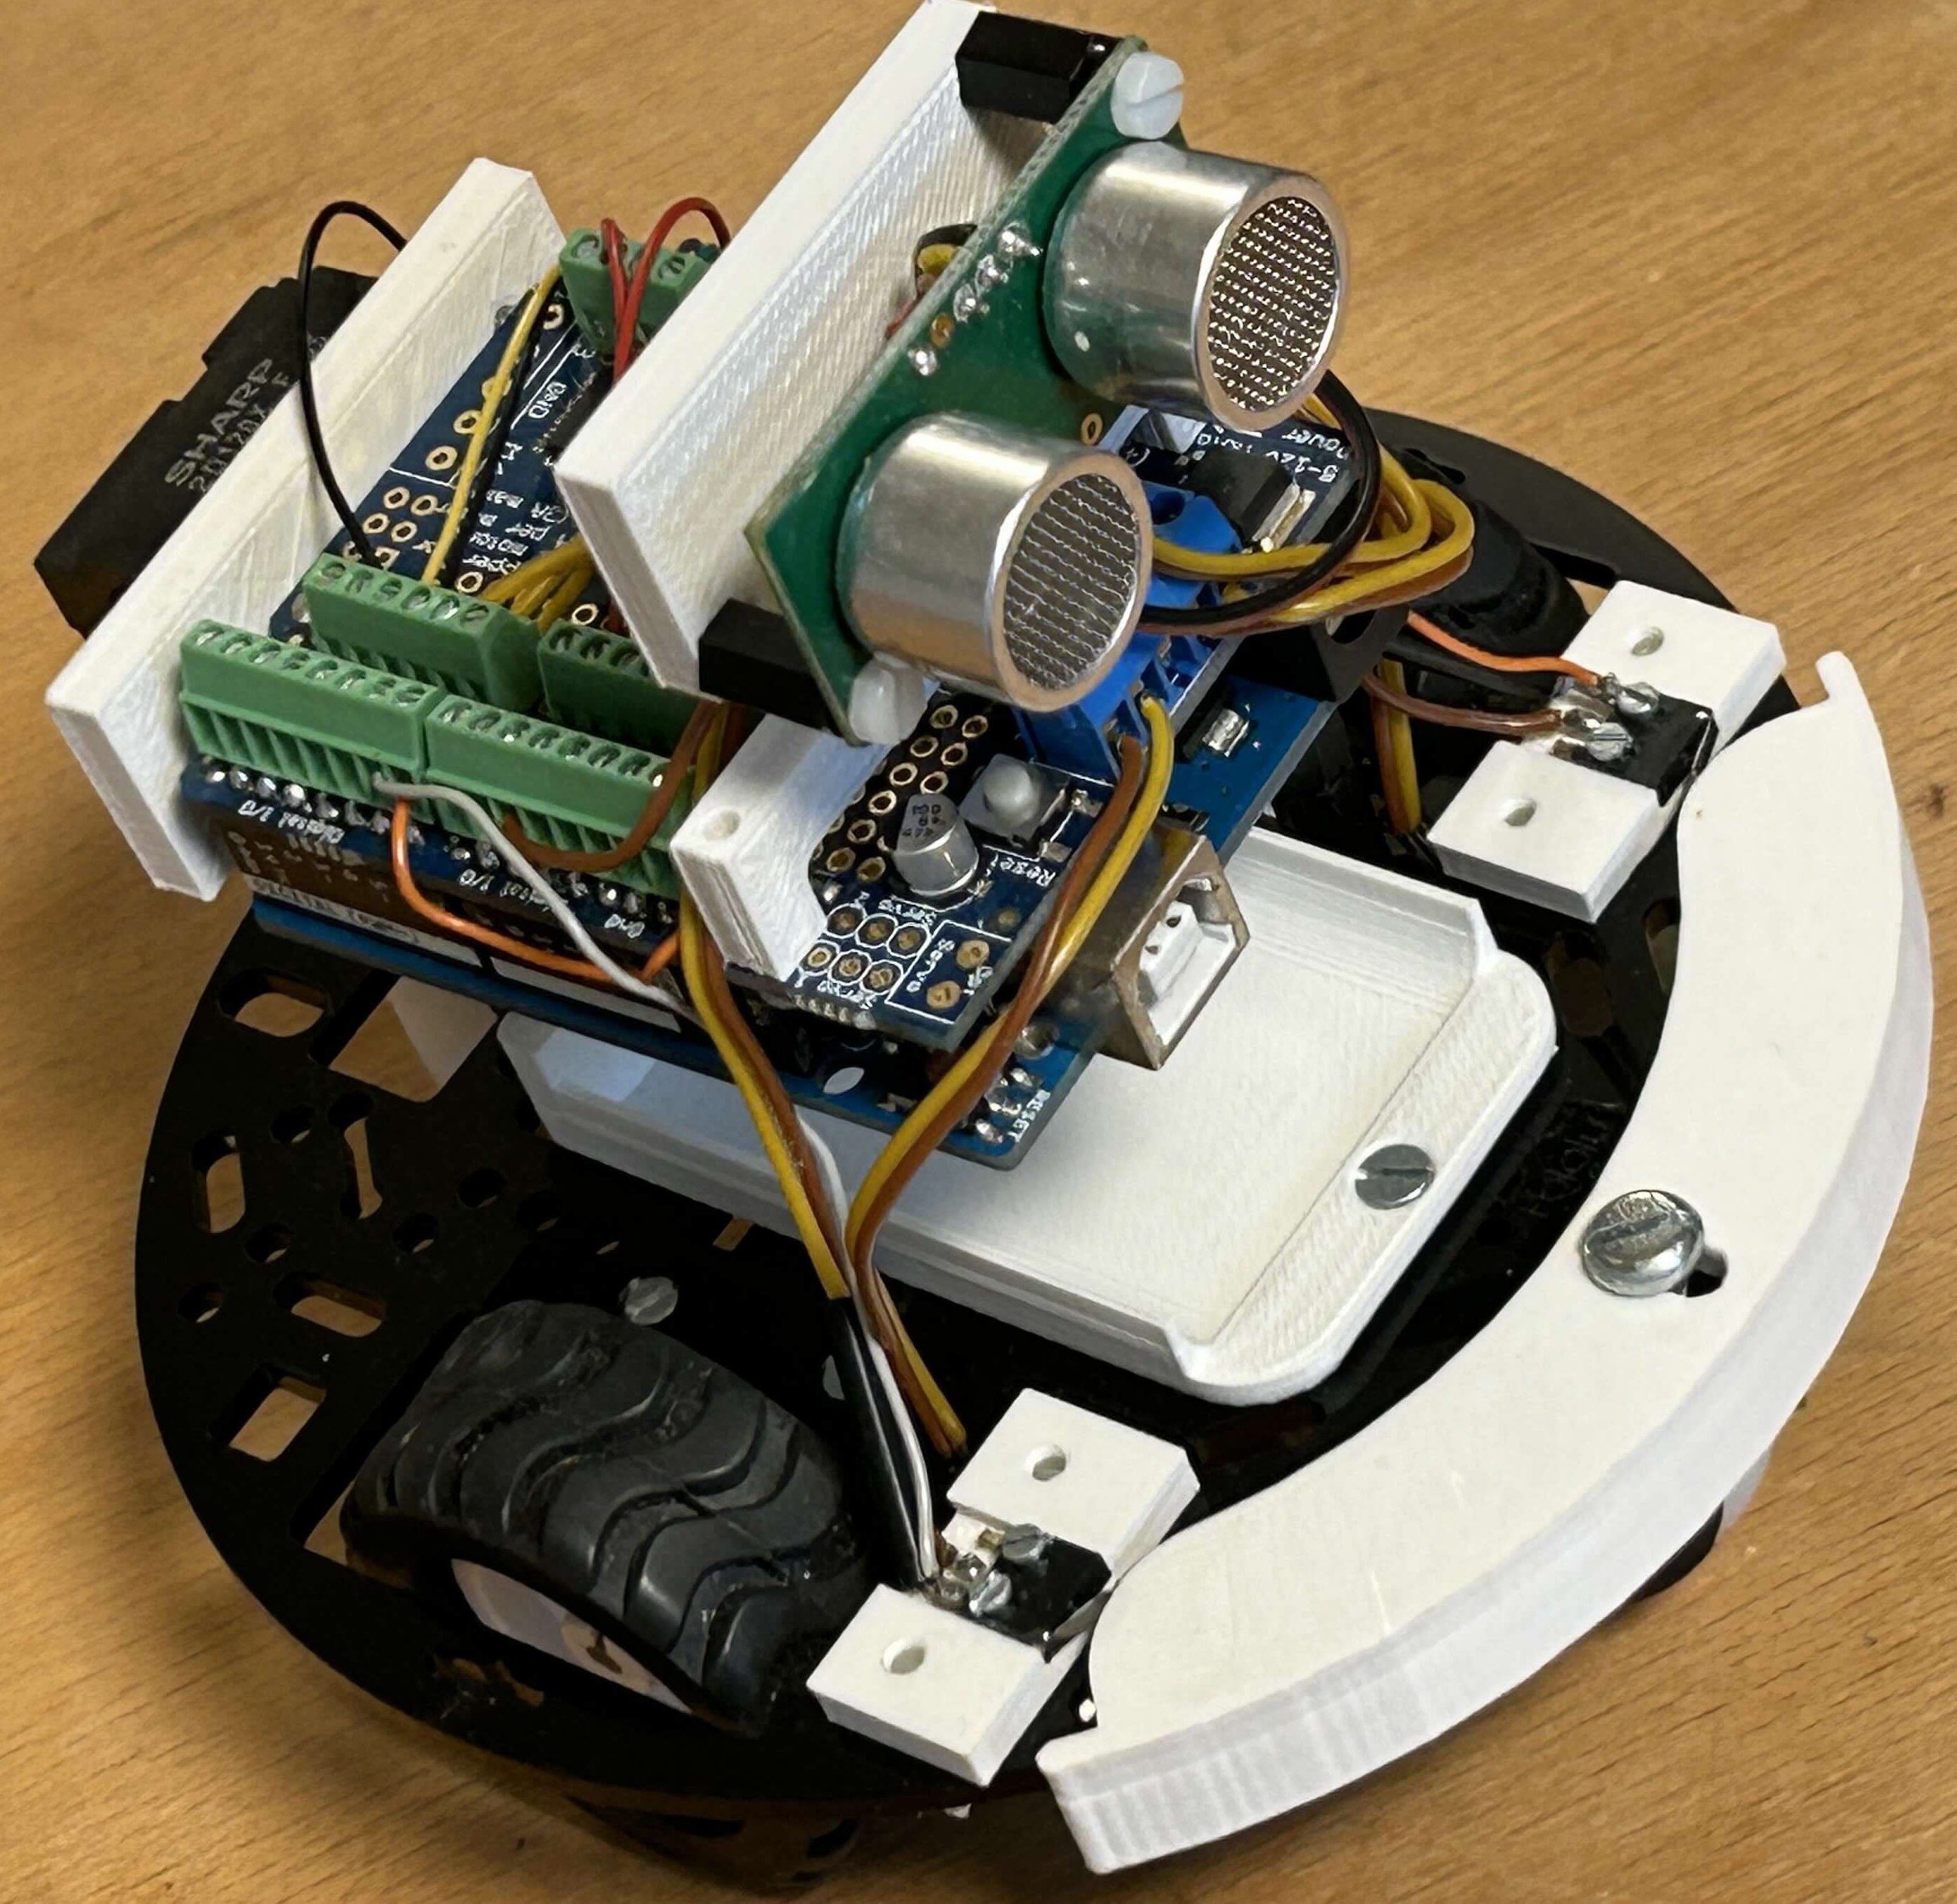
\includegraphics[width=.46\textwidth]{FF/Robotik/Skript/Abbildungen/arduino_roboter.jpg}
	\caption{Roboter mit Arduino, Motor Shield und Gleichstrommotoren.}
	\label{fig:arduino-robot}
\end{figure}

\begin{myexercise}
Programmieren Sie den Roboter so, dass er eine Linkskurve fährt, anhält, am Ort dreht, um zwei Gegenstände eine Acht und ein Quadrat mit ungefähr \qty{1}{\metre} Kantenlänge fährt. Untersuchen Sie den Einfluss von Geschwindigkeit, Batteriespannung und Untergrund.
\begin{myanswer}keine Musterlösung\end{myanswer}
\end{myexercise}

\begin{mysummary}\phantom{1}
\begin{itemize}
	\item Motoren benötigen eine geeignete externe Versorgung und eine gemeinsame Masse mit dem Arduino.
	\item Ein Positionsservo fährt mithilfe periodischer Steuerimpulse einen Winkel an.
	\item Ein Motor Shield steuert Drehrichtung und Geschwindigkeit von Gleichstrommotoren.
\end{itemize}
\end{mysummary}
